\begin{frame}
    \centering
    \Huge Paradigma NoSQL

\end{frame}

\begin{frame}
    \frametitle{Paradigma NoSQL}

    \centering
    \Huge NoSQL \only<1>{$=$ ?`?}\only<2>{$\neq$ No to SQL}\only<3>{$=$ Not only SQL}

\end{frame}

\begin{frame}
    \frametitle{ACID vs. BASE}

    \centering
    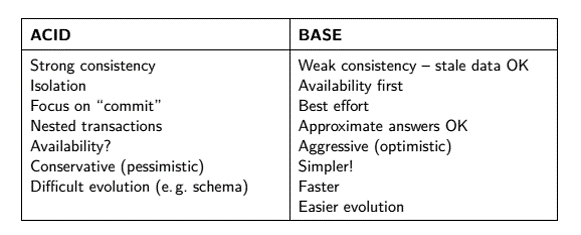
\includegraphics[width=\textwidth]{acid-vs-base.jpg}
\end{frame}

\begin{frame}
    \frametitle{SBD NoSQL}

    \begin{block}{Usos frecuentes}
        \pause
        \begin{itemize}[<+->]
            \item Escenarios con nuevos problemas en la organización
            \item Carga de los datos previa a conocer el esquema o con gran variación
            \item Contextos donde las BDRs no aseguran  el desempeño requerido para manipular los datos actuales
            \item Dinamismo en la definición de las interrelaciones
            \item Necesidad de distribución y acceso global
        \end{itemize}
    \end{block}

\end{frame}

\begin{frame}
    \frametitle{SBD NoSQL}

    \begin{columns}
        \column{0.5\textwidth}
        \begin{exampleblock}{Pros}
        \begin{itemize}
            \item Escalabilidad
            \item Flexibilidad
            \item Alto Rendimiento
            \item Agilidad
            \item Adecuado para Big Data y aplicaciones en tiempo real
        
        \end{itemize}
        \end{exampleblock}
        
        \column{0.5\textwidth}
        \begin{alertblock}{Contras}
        \begin{itemize}
            \item Problemas de consistencia
            \item Complejidad
            \item Limitaciones de consultas
            \item Soporte limitado de transacciones
            \item Desafíos en Consistencia e Integridad de Datos
        \end{itemize}
        \end{alertblock}
        
    \end{columns}
\end{frame}